\documentclass[a4paper,10pt]{article}

\usepackage{graphicx}
\usepackage[latin1]{inputenc}
\usepackage[spanish]{babel}

\title{ \textbf{ 6620. Organizaci\'on de Computadoras
Trabajo Pr\'actico 2: Optimizaci\'on de Software}}

\author{	Gonz\'alez, Juan Manuel, \textit{Padr\'on Nro. 79.979} \\
            	\texttt{ juan0511@yahoo.com } \\[2.5ex]
		Smocovich, Elizabeth, \textit{Padr\'on Nro. 86.326} \\
            	\texttt{ liz.smocovich@gmail.com } \\[2.5ex]
            	Pereira, Mar\'ia Florencia, \textit{Padr\'on Nro. 88.816} \\
            	\texttt{ mflorenciapereira@gmail.com } \\[2.5ex]
            	\normalsize{1er. Cuatrimestre de 2010} \\
            	\normalsize{66.20 Organizaci\'on de Computadoras  $-$ Pr\'atica Jueves} \\
            	\normalsize{Facultad de Ingenier\'ia, Universidad de Buenos Aires} \\
       }
\date{}

\begin{document}
\maketitle
\thispagestyle{empty}  % quita el nmero en la primer pagina

\begin{abstract}
El presente trabajo tiene como objetivo aplicar optimizaciones de software en ambientes reales y familiarizarse con la medici\'on de comportamiento utilizando herramientas de \textit{profiling}.
\end{abstract}

\pagebreak

\pagestyle{empty}
\section{Introducci\'on}
Un algoritmo de la multiplicaci\'on de matrices en lenguaje C sencillo, pero ineficiente en cuanto a la utilizaci\'on de la memoria cache es la siguiente:

\begin{verbatim}
for(i=0;i<N;i++)
    for(j=0;j<M;j++)
        for(k=0;k<L;k++)
            c[i][j]+=a[i][k]*[k][j];
\end{verbatim}

Este programa multiplica las matrices \textit{A} $\in \Re{R}^{NxL}$ y \textit{B} $\in \Re^{LxM}$, dando como resultado una matriz \textit{C} $\in \Re^{NxM}$. Al recorrer una de las matrices por filas y la otra por columnas, para matrices mayores que la memoria cache se producir\'an ineficiencias a la hora de operar con ella.\\
En el presente trabajo se hara uso de las t\'ecnicas de optimizaci\'on de uso de la memoria cache vistas en el curso, modificando un programa que resuelve una multiplicaci\'on de dos matrices. Se buscar\'a reducir la cantidad de desaciertos (\textit{misses}) en la memoria cach\'e de datos de nivel 1 (L1) y el tiempo de ejecuci\'on . Para esto se utilizar\'a el m\'odulo de simulaci\'on de memorias cach\'e, llamado Cachegrind, e integrado a Valgrind y la herramienta de profiling gprof. Las optimizaciones a aplicar ser\'an \textit{padding},  \textit{blocking} y \textit{prefetch}.

\section{Consideraciones sobre el desarrollo e implementaci\'on}
A continuaci\'on se detallan las consideraciones tenidas en cuenta para el desarrollo del trabajo pr\'actico. 

En esta secci\'on se discutir\'an los m\'etodos de optimizaci\'on que fueron implementados en la versi\'on final del trabajo pr\'actico. Tambi\'en se expondr\'an los resultados obtenidos de las mejoras introducidas en el c\'odigo, basados en las pruebas realizadas seg\'un se expone en la secci\'on 3.

\subsection{Elecci\'on del nivel de memoria a optimizar}
Para reducir la brecha de velocidad entre el procesador y la memoria f\'isica,
la arquitectura de las computadoras suele incluir varios niveles de memoria. Las memorias caches multi-nivel operan 
revisando la memoria L1 primero. Si se produce un miss, a continuaci\'on se revisa la cache L2 y as\'i sucesivamente con los niveles siguientes 
hasta la memoria f\'isica. Las memorias cache grandes tienen un porcentaje alto de hit rate pero una latencia mayor. El primer nivel de memoria 
es peque\~no para que los ciclos que se consuman sean comparables con los ciclos de reloj del CPU. La memoria cache de nivel 2 es de mayor tama\~no para 
capturar gran parte de los accesos a memoria, disminuyendo as\'i el \textit{miss penalty}. Dado el tama\~no de la memoria L1, es probable que su miss rate sea mayor que 
el de la memoria L2.  Por esta raz\'on, se decidi\'o optimizar el c\'odigo para la memoria cache L1, ya que si se redujera el miss rate de este nivel, el tiempo de 
ejecuci\'on ser\'ia menor. Para la memoria cache L2 esto no ser\'ia posible ya que el miss rate es bastante menor que el de la L1 y la latencia no 
es una caracter\'istica que pueda optimizarse por software.

\subsection{Optimizaci\'on del algoritmo y resultados}

A fin de mejorar el rendimiento, se ensayaron tres soluciones:\\

\subsubsection*{Padding}
Se conoce como \textit{Padding} al agregado de variables sin usar entre dos \textit{arrays} para reducir la interferencia entre ellos y de esta forma mejorar la tasa de \textit{miss}. Agregar un \textit{pad} modifica el \textit{offset} del segundo \textit{array}, por lo que se puede lograr que estos queden mappeados en distintas partes de la cache, evitando as\'i conflictos. El taman\~os de los \textit{pad} depende del esquema de \textit{mappeo} de la memoria cache, su grado de asociatividad y el patr\'on de acceso a los datos del c\'odigo. Valores t\'ipicos suelen ser m\'ultiplos de del tama\~no de l\'inea.
De esta manera, se logra evitar el acceso a datos distintos ubicados en la misma posici\'on de memoria cache (\textit{thrashing}).
Esta optimizaci\'on cambia la forma en que los arreglos son almacenados en memoria principal, reduciendo los accesos conflictivos. Una desventaja es que utiliza mayor cantidad de memoria.\\
En cuanto a los resultados obtenidos mediante esta t\'ecnica, no se observ\'o una mejora significativa en la ejecuci\'on del algoritmo. Esto puede deberse a que el tama\~no de la matriz sobre la que 
estamos operando tiene dimensi\'on de N x N donde N=576, que para la arquitectura donde se llevaron a cabo las pruebas, era m\'ultiplo del tama\~no de la l\'inea de cache (64 bytes). \\
\begin{center}
 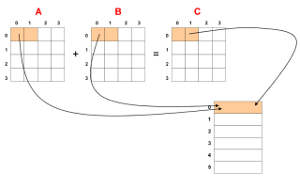
\includegraphics[width=200px,height=100px]{./padding1.png}
 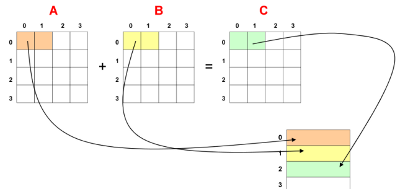
\includegraphics[width=200px,height=100px]{./padding2.png}

 % ssh1.png: 408x340 pixel, 96dpi, 11.59x9.79 cm, bb=0 0 328 277
\end{center}







\subsubsection*{Loop blocking o tiling}
\begin{center}
 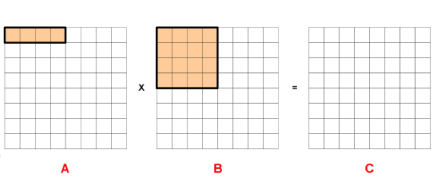
\includegraphics[width=200px,height=95px,scale=1]{./blocking.png}
  % ssh1.png: 408x340 pixel, 96dpi, 11.59x9.79 cm, bb=0 0 328 277
\end{center}

\textit{Loop blocking} es una transformaci\'on de los ciclos en los cuales se incrementa su profundidad. Si la profundidad original es n, el resultado podr\'a ser de cualquier profundidad entre n+1 y 2n. Se busca mediante este m\'etodo resolver mejor la localidad de los datos, para que la mayor\'ia de ellos se encuentren en el cache en el momento y orden que se pretende leerlos de memoria.
Esta t\'ecnica permite decrementar la cantidad de desaciertos de capacidad cuando se opera con arreglos grandes y mejora la localidad temporal (mantiene en la cache, datos que se usar\'an en el corto plazo). Asimismo, se reducen los accesos conflictivos, ya que los bloques
peque\~nos pueden ser mantenidos en la cache. \\
Para esta optimizaci\'n existe un par\'ametro llamado blocking factor (B). Este factor deber\'a ser elegido para que las submatrices B x B entren completamente en la memoria cache. 
En la pr\'actica, si bien al variar este par\'ametro se produc\'ia una reducci\'on importante en la tasa de miss, esto no suced\'ia con el tiempo de ejecuci\'on. Una explicaci\'on para esto
es que si bien se reducen la cantidad de miss en el total de accesos, al incorporara m\'as lazos se ejecutar\'an mayor cantidad de instrucciones, lo cual hace incrementar los ciclos. de ejecuci\'on.

\subsubsection*{Software prefetch}
\textit{Software prefet} es una t\'ecnica de optimizaci\'on que especula con los accesos futuros a datos e instrucciones. El obtjetivo es traer a la memoria cache los datos que 
se necesitar\'an en el futuro, al mismo tiempo que se precesarn los datos actuales. En lenguaje C, es posible realizar una lectura
adelantada mediante \textit{\_\_builtin\_prefetch()}, si la arquitectura lo soporta. 
La operaci\'on de prefetch es de tipo \textit{non-blocking}, raz\'on por la cual para poder implementar software prefetching se deber\'a contar con una arquitectura 
que permita al procesador continuar funcionando mientrar se realiza la operaci\'on. 
\textit{Software prefetching} suele utilizarse frecuentemente cuando se tienen lazos de gran dimensi\'n dado que exhiben un patr\'on predecible de accesos.
Para aplicar esta t\'ecnica se dividi\'o el lazo correspondiente a la matriz A (que se recorre por filas) en 3 partes: pr\'ologo, procesamiento principal y ep\'ilogo. En el pr\'ologo se 
traen tantos elementos como entren en una l\'inea de cache. En el procesamiente principal, se traen a memoria los siguientes datos y se procesan los que ya se se encuentran en ella. 
Finalmente, en el ep\'ilogo se termina de procesar los \'ultimos datos. No se aplic\'o prefetch a la matriz B porque, al ser \'esta recorrida por columnas, siempre producir\'a un miss dada la estructura de la memoria.
Un par\'ametro configurable de esta t\'ecnica es la distance de prefetch D, que es igual a la cantidad de bloques le\'idos en forma adelantada dividida la cantidad de bloques preocesados. Otra definici\'on 
dice que la distancia D = l/s donde l es la latencia promedio de la memoria y s la cantidad de ciclos estimado de la iteraci\'on m\'as r\'apida del lazo.
Tomamos D=8 dado que los resultados fueron mejores para la arquitectura donde se realizaron las pruebas. Un aspecto importante es que esta optimizaci\'on permiti\'o reducir el tiempo de 
ejecuci\'on significativamente, solucionando el problema mencionado anteriormente en la descripci\'on de \textit{Loop blocking}.






\subsubsection*{Otras mejoras posibles}

Otras opciones para optimizar a\'un mas el algoritmo, fuera del alcance de nuestra implementaci\'on, incluyen por ejemplo el uso de alineaci\'on de datos (\textit{data alignment}), que evita la fragmentaci\'on de los datos en la cach\'e.\\
Otra posible optimizaci\'on ser\'ia loop fusion que aplica a lazos con el mismo espacio de iteraci\'on una transformaci\'on que fusiona los cuerpos de cada lazo en uno solo.


\section{Instalaci\'on}
A continuaci\'on se detallan los pasos para instalar y ejecutar el trabajo pr\'actico
\begin{enumerate}
 \item Descomprimir el archivo TP2.tar.gz en una carpeta.
\item 
En un terminal, dentro de la carpeta del paso anterior, escribir ./instalar.
\item 
En un terminal, dentro de la carpeta del paso anterior, escribir ./tp2 [opciones].
\end{enumerate}





\section{Corridas de prueba}

En esta secci\'on se presentan, a modo demostrativo, algunas de las corridas efectuada para probar el funcionamiento del trabajo pr\'actico\\
Tambi\'en se comentan los resultados que se obtuvieron al variar los par\'ametros de cada optimizaci\'on
Las pruebas se realizaron para una memoria cache de datos, cuyas caracter\'isticas son:

\begin{itemize}
 \item \textbf{Cantidad de v\'ias:} 8
 \item \textbf{Tama\'no:} 32K
\item \textbf{Cantidad de sets:} 64
\end{itemize}


\subsection*{Padding}
\begin{itemize}
\item pad=2*(tama\~no de la l\'inea)\end{itemize}

\begin{center}
 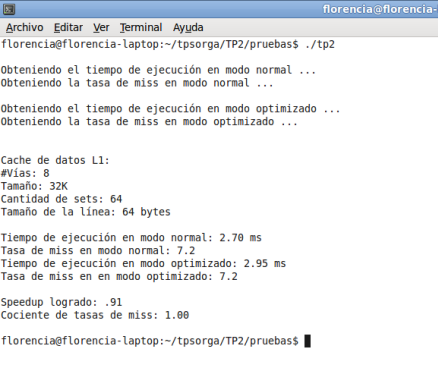
\includegraphics[width=250px,height=200px,bb=0 0 328 277,scale=1]{./ssh1.png}
 % ssh1.png: 408x340 pixel, 96dpi, 11.59x9.79 cm, bb=0 0 328 277
\end{center}




\subsection*{Padding}
\begin{itemize}
\item pad=4*(tama\~no de la l\'inea)\end{itemize}

\begin{center}
 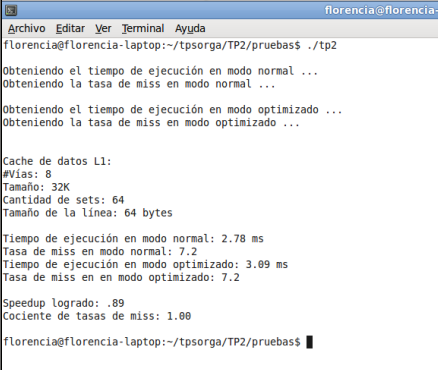
\includegraphics[width=250px,height=200px,bb=0 0 328 277,scale=1]{./ssh2.png}
 % ssh1.png: 408x340 pixel, 96dpi, 11.59x9.79 cm, bb=0 0 328 277
\end{center}


\subsection*{Padding}
\begin{itemize}
\item pad=8*(tama\~no de la l\'inea)
\end{itemize}

\begin{center}
 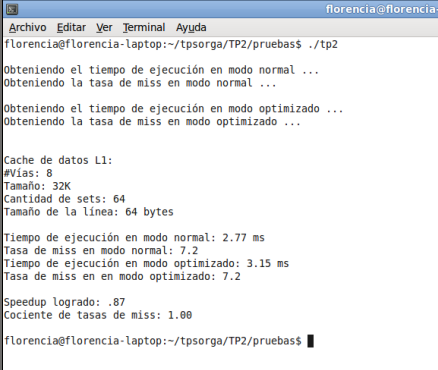
\includegraphics[width=250px,height=200px,bb=0 0 328 277,scale=1]{./ssh3.png}
 % ssh1.png: 408x340 pixel, 96dpi, 11.59x9.79 cm, bb=0 0 328 277
\end{center}


Como se mencion\'o anteriormente, no se observan cambios significativos al agregar padding a las matrices.\\


\subsection*{Padding y Blocking}
\begin{itemize}
 \item pad=2*tama\~no de la l\'inea
 \item B=2
\end{itemize}

\begin{center}
 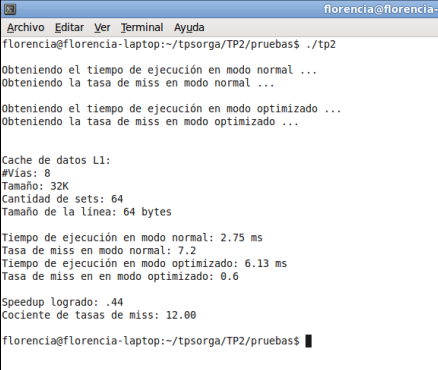
\includegraphics[width=250px,height=200px,bb=0 0 328 277,scale=1]{./ssh4.png}
 % ssh1.png: 408x340 pixel, 96dpi, 11.59x9.79 cm, bb=0 0 328 277
\end{center}

\subsection*{Padding y Blocking}
\begin{itemize}
\item Con pad=2*tama\~no de la l\'inea
\item B=4
\end{itemize}
\begin{center}
 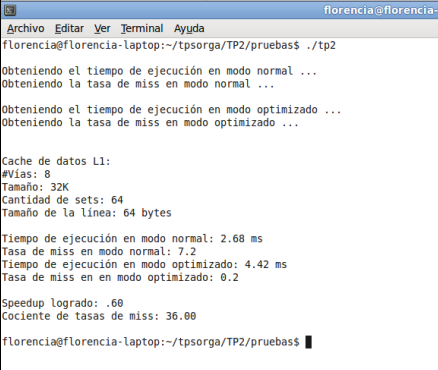
\includegraphics[width=250px,height=200px,bb=0 0 328 277,scale=1]{./ssh5.png}
 % ssh1.png: 408x340 pixel, 96dpi, 11.59x9.79 cm, bb=0 0 328 277
\end{center}


\subsection*{Padding y Blocking}
\begin{itemize}
\item pad=2*tama\~no de la l\'inea
\item B=(cache\_size)/8
\end{itemize}
\begin{center}
 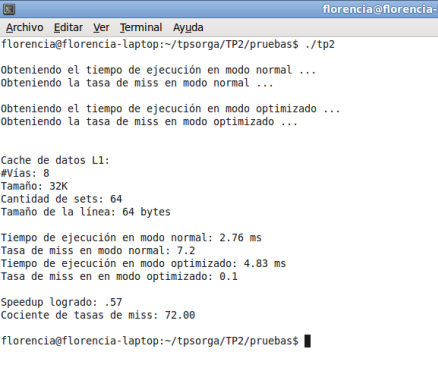
\includegraphics[width=250px,height=200px,bb=0 0 328 277,scale=1]{./ssh6.png}
 % ssh1.png: 408x340 pixel, 96dpi, 11.59x9.79 cm, bb=0 0 328 277
\end{center}


Podemos observar que el mientras m\'as grande sea B (siempre siendo menor al tama\'no de la memoria cache), disminuye m\'as la tasa de miss.
Sin embargo, el tiempo de ejecuci\'on es mayor al original. Como se mencion\'o antes, esto puede deberse a que ahora se ejecutan m\'as instrucciones
por el agregado de m\'as lazos.
Para poder implementar prefetch, se tom\'o B=(cache\_size)/8*D\\

\subsection*{Prefetch, Padding y Blocking}
\begin{itemize}
\item pad=2*tama\~no de la l\'inea
\item D=2
\item B=D*(cache\_size)/8
\end{itemize}

\begin{center}
 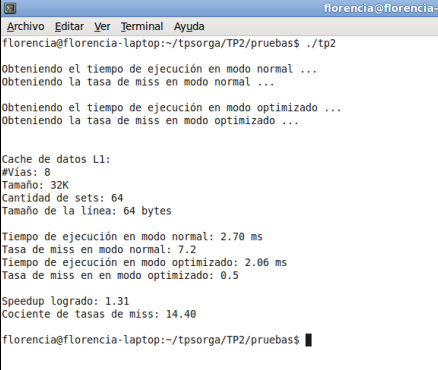
\includegraphics[width=250px,height=200px,bb=0 0 328 277,scale=1]{./ssh7.png}
 % ssh1.png: 408x340 pixel, 96dpi, 11.59x9.79 cm, bb=0 0 328 277
\end{center}


\subsection*{Prefetch, Padding y Blocking}
\begin{itemize}
\item pad=2*tama\~no de la l\'inea
\item D=4
\item B=D*(cache\_size)/8
\end{itemize}

\begin{center}
 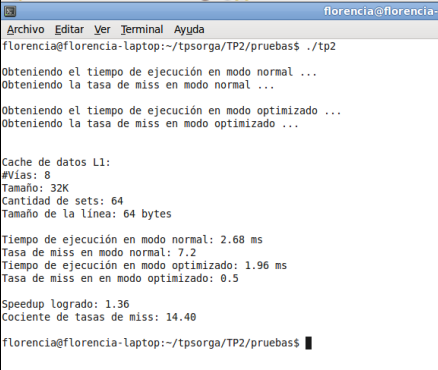
\includegraphics[width=250px,height=200px,bb=0 0 328 277,scale=1]{./ssh8.png}
 % ssh1.png: 408x340 pixel, 96dpi, 11.59x9.79 cm, bb=0 0 328 277
\end{center}


\subsection*{Prefetch, Padding y Blocking}
\begin{itemize}
\item pad=2*tama\~no de la l\'inea
\item D=8
\item B=D*(cache\_size)/8\end{itemize}
\begin{center}
 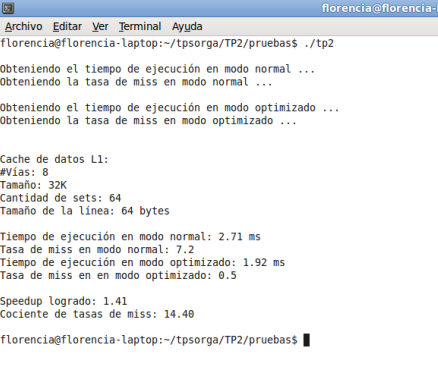
\includegraphics[width=250px,height=200px,bb=0 0 328 277,scale=1]{./ssh9.png}
 % ssh1.png: 408x340 pixel, 96dpi, 11.59x9.79 cm, bb=0 0 328 277
\end{center}



Observamos que con el aumento de la distancia de prefetch, mejora el tiempo de ejecuci\'on y la tasa de miss se mantiene constante.\\

Como conclusi\'on decidimos presentar esta \'ultima opci\'on dado que presenta una mejora importante tanto en el tiempo de ejecuci\'on como en la tasa de miss.











\pagebreak
\section{C\'odigo fuente original} 
\begin{verbatim}


 



\end{verbatim}

\pagebreak
\section{C\'odigo fuente modificado} 

A continuaci\'on se incluye el c\'odigo fuente del programa, con las modificaciones incorporadas.

\begin{verbatim}


\end{verbatim}



\pagebreak

\section{C\'odigo en shell script de instalar y tp2} 

A continuaci\'on se incluyen los  archivos ejecutables que realizan la instalaci\'on y medici\'on de tiempos de ejecuci\'on y miss rates.
\pagebreak


\section{Enunciado} 

A continuaci\'on se incluye el enunciado del tr\'abajo pr\'actico.
\pagebreak

\section{Conclusiones}

El estudio de la problem\'atica de la multiplicaci\'on entre matrices cuadradas gener\'o diversos algoritmos para su optimizaci\'on. Las condiciones que se presentan en la misma (saltos en la memoria principal, \textit{thrashing}, gran cantidad de ciclos) la vuelven ideal para tomarla como caso de estudio. Utilizando \textit{padding}, no logramos mejorar significativamente el rendimiento de la memoria cache al ejecutar la aplicaci\'on. Por otro lado, encarando la resoluci\'on del problema con la t\'ecnica de \textit{blocking} se logr\'o una importante mejora en el rendimiento, aunque no as\'i en el tiempo de ejecuci\'on. 
Finalemente, incluir \textit{software prefetch}  produce una mejora en este \'ultimo aspecto.\\
Al juntar todas las optimizaciones en un solo c\'odigo fuente, pudimos observar que se obtiene una mejora global. Es importante seleccionar los par\'ametros de cada optimizaci\'on de forma tal que se obtenga un mayor beneficio.
En definitiva, la multiplicaci\'on de matrices es una situaci\'on ideal para ejercitar los distintos m\'etodos de optimizaci\'on investigados.\\


A modo de conclusi\'on, podemos comentar que una vez concluidos los casos de prueba y luego de sendos testeos, notamos que se obtiene una mejora en el procesamiento y la aplicaci\'on hace mejor uso de los recursos del sistema.\\
\pagebreak




\begin{thebibliography}{99}

\bibitem{VALGRIND} Herramientas de profiling Valgrind. http://valgrind.org/

\bibitem{CACHE} The Cache Performace and Optimizations of Blocked Algorithms. Monica S. Lam an Edward E. Rothberg and Michael E. Wolf. Computer Systems Laboratory, Stanford University. http://suif.standford.edu/papers/lam91.ps

\bibitem{GCC} GCC: Online Documentation. http://gcc.gnu.org/onlinedocs/

\bibitem{LATEX} Oetiker, Tobias, ``The Not So Short Introduction To LaTeX2'', http://www.physics.udel.edu/$\sim$dubois/lshort2e/

\bibitem{LIBROC} Kernighan, Brian W. / Ritchie, Dennis M. \underline{El Lenguaje De Prorgamaci\'on C}. Segunda Edici\'on, PRENTICE-HALL HISPANOAMERICANA SA, 1991.

\bibitem{PATHEN} Patterson / Hennesy. \underline{Computer Organization and Design; The Hardware-Software Interface}. Second Edition. Morgan Kaufman, 1997.

\end{thebibliography}

\end{document}

